\documentclass[../SimBALink.tex]{subfiles}
\begin{document}

\subsection{Tires}
\subsection{Inputs and outputs}
	\subsubsection{Inputs}
	\begin{tabular}{ l | l | l  }
		Input					&	Symbol		&	Unit		\\	\hline
		Brake Force				& 	$F_b$ 		&	N \\
		Gear Torque				&	$\tau_g$	&	Nm \\
		Wheel Forces[3]			&	$F_w$		&	N[3] \\
		Vehicle Velocity		&	$v$			&	m/s \\
		Lead Angle				&	$\theta_l$	&	rad \\
	\end{tabular}
	
	\subsubsection{Outputs}
	\begin{tabular}{ l | l | l  }
		Output					&	Symbol		&	Unit		\\	\hline
		Tire Torque				&	$\tau_t$	&	Nm \\
		Tire Reaction Force		&	$F_t$		&	N \\
	\end{tabular}

\subsubsection{Background, rationale, modeling strategy} The tire is modeled in three parts, rolling resistance, Load and Torque, and Traction Limiting. Force directions are defined as longitudinal(long), lateral(lat), and normal(n). Longitudinal is along the direction of the motorcycle (when moving straight). Lateral is orthogonal to Longitudinal axis. Normal 3-D orthogonal to lateral and longitudinal, in general the axis to the road on no incline.

In general the tire model provides a load on the Gear/Chain and gives the vehicle a reaction force. Load is caused by the forces from the road(from the vehicle) and rolling resistance. the reaction force caused by traction limiting which is a function of wheel slip. The amount of reaction force i saturated at the maximum force the tire can apply given wheel slip.  

\begin{gather}
\notag \textbf{Rolling Resistance} \\
K_t = 
\left\{
  \begin{array}{lr}
    0.0085 + \frac{0.18}{p_t} + \frac{1.59*10^{-6}}{p_t} & : v_{kph} \le 165 (km/h)\\
    \frac{0.18}{p_t} + \frac{2.91*10^{-6}}{p_t} & : v_{kph} > 165 (km/h)
  \end{array}
\right. \\
\notag \textbf{Wheel Slip} \\
\kappa = \frac{v - \omega_t r_t(\theta_l)}{v} \\
\mu_{t,gnd} = D_{\kappa}\sin(C_{\kappa} \arctan[B_{\kappa}\kappa - E_{\kappa}(B_{\kappa}\kappa - \arctan B_{\kappa}\kappa)]) \\
\notag \textbf{Load and Torque} \\
\tau_t = \tau_g - F_{w,long}r_t(\theta_l) - F_br_b - K_t F_{w,n} v_{kph}^2 \\
\notag \textbf{Traction Limiting} \\
F_{max} = \mu_{t,gnd} F_{w,n} \\
F = \tau r_t((\theta_l) \\
F_t =
\left\{
  \begin{array}{lr}
	F & : -F_{max} \le F \le F_{max} \\
	F_{max} & : -F_{max} > F > F_{max}
  \end{array}
\right. 
\end{gather}

The tire coefficient ($\mu_{t,gnd}$) is modeled using the "Magic Formula" as shown below. Where $D_{\kappa}$ is the maximum tire coefficient of the tire. 

 \begin{figure}[h!]
  \centering
  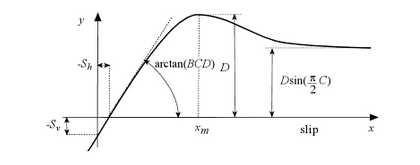
\includegraphics[scale=1]{magic_formula}
  \caption{Magic Formula }
\end{figure}

\subsubsection{Variables}
	\begin{tabular}{ l | l | l  }
		Var					&	Symbol		&	Unit		\\	\hline
		Tire Pressure		&	$p_t$		&	 $bar$ \\
		Brake Caliper Radius &	$r_b$		&	m \\
	\end{tabular}
\subsubsection{Parameters}
	\begin{tabular}{ l | l | l  }
		Param.					&	Symbol		&	Unit		\\	\hline
		 Magic Formula\\		&	$A_{\kappa},B_{\kappa},C_{\kappa},D_{\kappa}$		&	 n/a \\
	\end{tabular}
	
\subsubsection{Function}
$r_t(\theta_l)$ \\
	\begin{tabular}{ l | l | l | l }
		Type				& Description		&	Symbol		&	Unit		\\	\hline
		Input 				& Lean Angle		&	$\theta_l$  & 	rad		\\
		Output 				& Tire Radius		&	n/a			&	m
	\end{tabular} \\

\subsubsection{Assumptions}
\begin{itemize}
  \item Maximum acceleration force should also depend on lateral forces on the vehicle. However this is not modeled because it requires modeling of high-side and low-side dynamics. The Rider model should control for a safe operating area of the motorcycle to compensate for this assumption. 
  \item No tire deformation
  \item No tire temperature dynamics
  \item No change in rolling resistance with lean angle 
\end{itemize}


\end{document}